\documentclass{article}
\usepackage{amsmath}
\usepackage{amssymb}
\usepackage{graphicx}
\usepackage{hyperref}
\usepackage[version=4]{mhchem}


\begin{document}
\section*{Problem}
In \(\triangle A B C, \angle B A D=90^{\circ} . \angle D A C=45^{\circ} . A D\) is the median. Prove: \(A B\) \(=2 A D\).\\
\centering
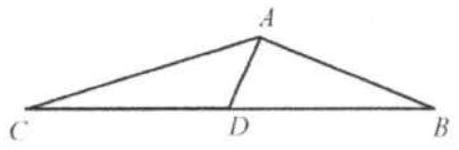
\includegraphics[width=\textwidth]{images/027(3).jpg}

\section*{Solution}
Extend \(A D\) to \(E\) such that \(A D=D E\).\\
Connect CE.\\
Since \(D E=A D, \angle C D E=\angle B D A . C D=D B\).\\
Thus \(\triangle C D E \cong \triangle B D A, C E=A B\), and \(\angle E=\angle D A B\) \(=90^{\circ}\).

Since \(\angle C A D=45^{\circ}\), in right triangle \(A E C, \angle A C E=\) \(45^{\circ}\).\\
\centering
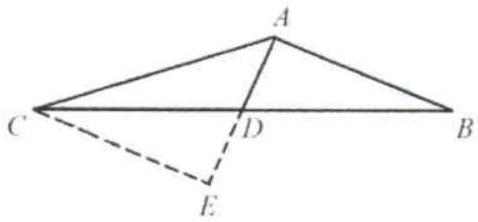
\includegraphics[width=\textwidth]{images/029.jpg}

Thus, \(C E=A E=2 A D\).\\
Since \(C E=A B, A B=2 A D\).

\end{document}
